\documentclass{beamer}

\usepackage{préambule}

\begin{document}

\begin{frame}
	\textbf{Recopie le diagramme suivant :}

	\begin{center}
		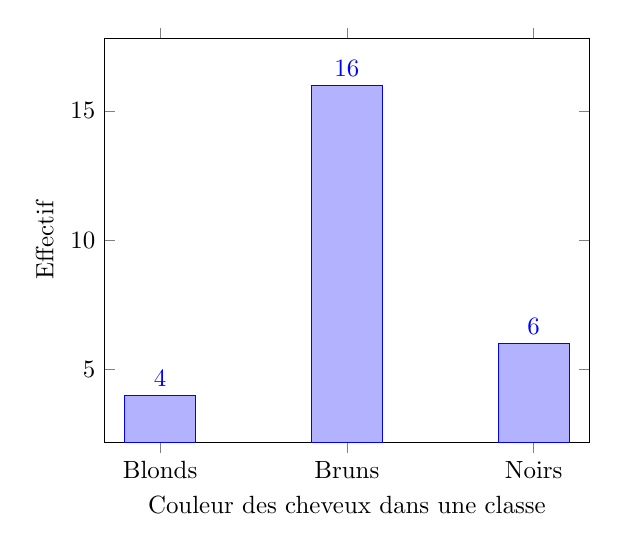
\begin{tikzpicture}[scale=0.9]
			\begin{axis}
				[
					ybar,
					bar width=1cm,
					enlargelimits=0.15,
					ylabel={Effectif},
					xlabel={\uline{Couleur des cheveux dans une classe}},
					symbolic x coords={Blonds, Bruns, Noirs},
					xtick=data,
					nodes near coords,
					nodes near coords align={vertical},
				]
				\addplot coordinates {(Blonds,4) (Bruns,16) (Noirs,6) };
			\end{axis}
		\end{tikzpicture}
	\end{center}

	Combien y-a-t'il d'élèves au total ? \dotfill

	Combien y-a-t'il d'élèves blonds ? \dotfill

	Quelle est la couleur de cheveux la plus répandue ? \dotfill
\end{frame}

\end{document}